\documentclass{article} % For LaTeX2e
\usepackage{nips14submit_e,times}
\usepackage{amsmath}
\usepackage{amsthm}
\usepackage{amssymb}
\usepackage{mathtools}
\usepackage{hyperref}
\usepackage{url}
\usepackage{algorithm}
\usepackage[noend]{algpseudocode}
%\documentstyle[nips14submit_09,times,art10]{article} % For LaTeX 2.09

\usepackage{mathrsfs}
\usepackage{graphicx}
\usepackage{caption}
\usepackage{subcaption}

\def\eQb#1\eQe{\begin{eqnarray*}#1\end{eqnarray*}}
\def\aB#1\aE{\begin{align*}#1\end{align*}}
\def\eQnb#1\eQne{\begin{align}#1\end{align}}
\providecommand{\e}[1]{\ensuremath{\times 10^{#1}}}
\providecommand{\pb}[0]{\pagebreak}

\newcommand{\E}{\mathrm{E}}
\newcommand{\Var}{\mathrm{Var}}
\newcommand{\Cov}{\mathrm{Cov}}

\def\Qb#1\Qe{\begin{question}#1\end{question}}
\def\Sb#1\Se{\begin{solution}#1\end{solution}}

\usepackage{scalerel,stackengine}
\stackMath
\newcommand\reallywidehat[1]{%
\savestack{\tmpbox}{\stretchto{%
  \scaleto{%
    \scalerel*[\widthof{\ensuremath{#1}}]{\kern-.6pt\bigwedge\kern-.6pt}%
    {\rule[-\textheight/2]{1ex}{\textheight}}%WIDTH-LIMITED BIG WEDGE
  }{\textheight}% 
}{0.5ex}}%
\stackon[1pt]{#1}{\tmpbox}%
}

\def\Xint#1{\mathchoice
    {\XXint\displaystyle\textstyle{#1}}%
    {\XXint\textstyle\scriptstyle{#1}}%
    {\XXint\scriptstyle\scriptscriptstyle{#1}}%
    {\XXint\scriptscriptstyle\scriptscriptstyle{#1}}%
      \!\int}
\def\XXint#1#2#3{{\setbox0=\hbox{$#1{#2#3}{\int}$}
    \vcenter{\hbox{$#2#3$}}\kern-.5\wd0}}
\def\dashint{\Xint-}

\newenvironment{claim}[1]{\par\noindent\underline{Claim:}\space#1}{}
\newtheoremstyle{quest}{\topsep}{\topsep}{}{}{\bfseries}{}{ }{\thmname{#1}\thmnote{ #3}.}
\theoremstyle{quest}
\newtheorem*{definition}{Definition}
\newtheorem*{theorem}{Theorem}
\newtheorem*{lemma}{Lemma}
\newtheorem*{question}{Question}
\newtheorem*{preposition}{Preposition}
\newtheorem*{exercise}{Exercise}
\newtheorem*{challengeproblem}{Challenge Problem}
\newtheorem*{solution}{Solution}
\newtheorem*{remark}{Remark}
\usepackage{verbatimbox}
\usepackage{listings}
\title{PDE-Evans}


\author{
Youngduck Choi \\
CIMS \\
New York University\\
\texttt{yc1104@nyu.edu} \\
}


% The \author macro works with any number of authors. There are two commands
% used to separate the names and addresses of multiple authors: \And and \AND.
%
% Using \And between authors leaves it to \LaTeX{} to determine where to break
% the lines. Using \AND forces a linebreak at that point. So, if \LaTeX{}
% puts 3 of 4 authors names on the first line, and the last on the second
% line, try using \AND instead of \And before the third author name.

\newcommand{\fix}{\marginpar{FIX}}
\newcommand{\new}{\marginpar{NEW}}

\nipsfinalcopy % Uncomment for camera-ready version

\begin{document}


\maketitle

\begin{abstract}
This work contains solutions to some 
problems in Evan's PDE.
\end{abstract}

\bigskip

\begin{question}[2-1]
\hfill
\begin{figure}[h!]
  \centering
    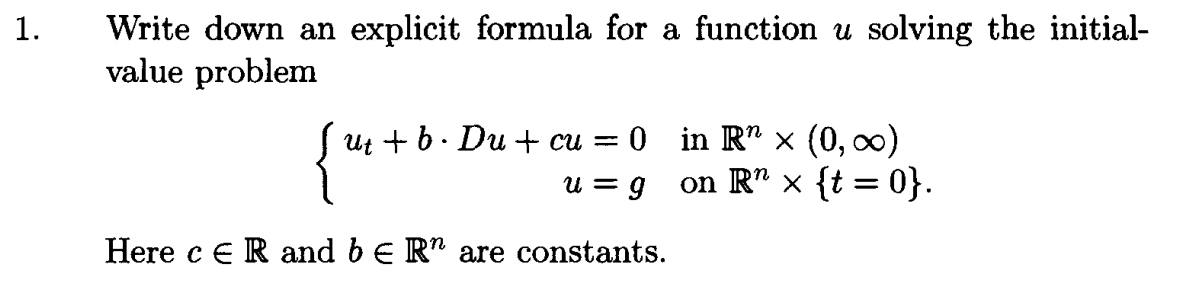
\includegraphics[width=0.8\textwidth]{evans-2-1.png}
\end{figure}
\end{question}

\begin{solution}
\end{solution}

\newpage

\begin{question}[2-2]
\hfill
\begin{figure}[h!]
  \centering
    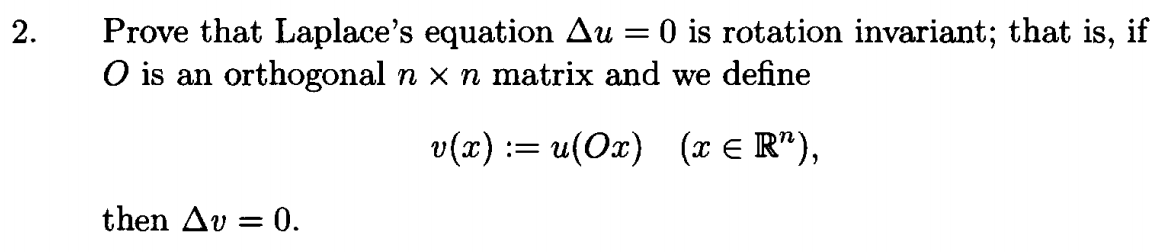
\includegraphics[width=0.8\textwidth]{evans-2-2.png}
\end{figure}
\end{question}


\begin{solution}
\end{solution}

\newpage

\begin{question}[2-3]
\hfill
\begin{figure}[h!]
  \centering
    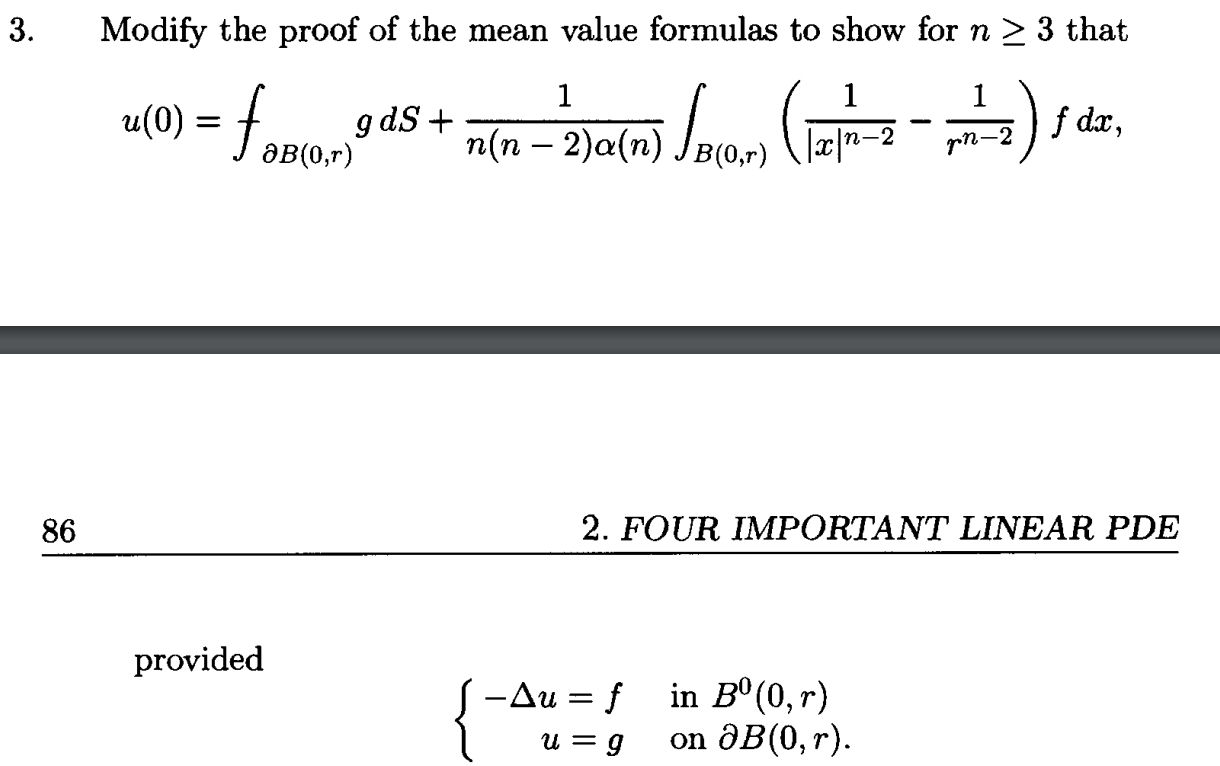
\includegraphics[width=0.8\textwidth]{evans-2-3.png}
\end{figure}
\end{question}

\begin{solution}
\end{solution}


\newpage

\begin{question}[2-4]
\hfill
\begin{figure}[h!]
  \centering
    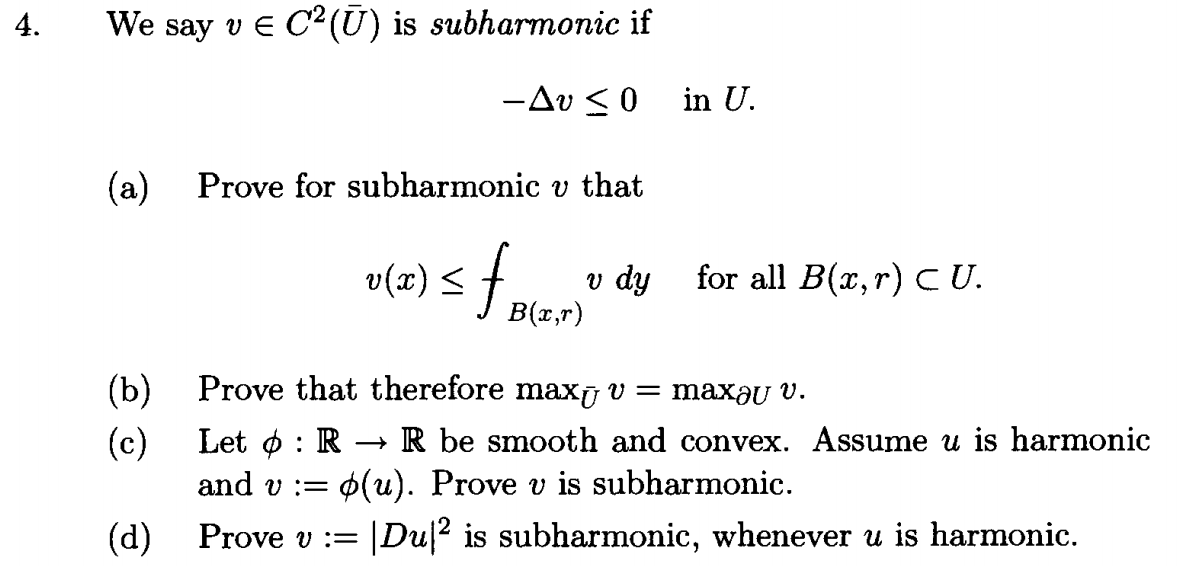
\includegraphics[width=0.8\textwidth]{evans-2-4.png}
\end{figure}
\end{question}
\begin{solution} $\>$ \\ 
\textbf{(a)} Fix $x \in U$. Define $\phi:(0,\text{dist}(x,\partial U)) \to \mathbb{R}$
by  
\eQb
\phi(r) &\vcentcolon =& \Xint-_{\partial B(x,r)} v(y)dS(y) = \Xint-_{\partial B(0,1)}
u(x+rz) dS(z).
\eQe
Then
\eQb
\phi'(r) &=& \Xint-_{\partial B(0,1)} Dv(x+rz) \cdot z dS(z), 
\eQe
and by Green's formula 
\eQb
\phi'(r) &=& \Xint-_{\partial B(x,r) } Dv(y) \cdot \dfrac{ y- x}{r} dS(y) \\
&=& \Xint-_{\partial B(x,r)} \dfrac{\partial v}{\partial \nu} dS(y) \\
&=& \dfrac{r}{n} \Xint-_{B(x,r)} \Delta v(y) dy. 
\eQe
Since $\Delta v \geq 0  \>\> \text{in} \>\> U$, the above equality implies
\eQb
\phi'(r) \geq 0 \>\> \text{in} \>\>  (0,\text{dist}(x,\partial U)). 
\eQe
so for a fixed $B(x,r_0) \subset U$, 
\eQb
v(x) = \lim_{r \to 0; \in (0,\text{dist}(x,\partial U))} \phi(r) 
\leq \Xint-_{\partial B(x,r_0)} v(y) dS(y). 
\eQe

\smallskip

2. Now employing polar coordinates yields, for any $B(x,r) \subset U$, 
\eQb
\int_{B(x,r)} v dy &=& \int_{0}^{r} \left( \int_{\partial B(x,r)} 
v dS \right) ds \\
&\geq& v(x) \int_{0}^{r} n\alpha(n) s^{n-1} ds = \alpha(n) r^n v(x),
\eQe
so 
\eQb
\Xint-_{B(x,r)} v dy &\geq& v(x),
\eQe
as required.

\textbf{(c)}
1. We assert that the converse of the sub-harmonic mean-value property
holds. Let $v \in C^2(\overline{U})$ such that 
\eQb
v(x) \leq \Xint-_{B(x,r)} v dy \>\> \text{ for all} \>\> B(x,r) \subset U.
\eQe 
If $\Delta v < 0$, by the $C^2$ smoothness of $v$,
there exists some ball $B(x,r_0) \subset U$ such that 
$\Delta v < 0$ within $B(x,r_0)$. But then for $\phi$ as above, and
$r \in (0,r_0)$,
\eQb
\phi'(r) &=& \dfrac{r}{n} \Xint-_{B(x,r)} \Delta u(y) dy < 0.
\eQe
This implies that
\eQb
v(x) = \lim_{r \to 0; r \in (0,r_0)} \phi(r)  > \Xint-_{B(x,r_0)} v dy,
\eQe
a contradiction.

\bigskip
2. Fix $x \in U$ and $B(x,r) \subset U$. Observe that $B^{0}(x,r)$ 
is open, bounded, and 
$u$ is harmonic, thus summable. Thus by Jensen's inequality,
and the mean value property of $u$, we obtain
\eQb
\Xint-_{B(x,r)} v dx &=&
\Xint-_{B^0(x,r)} v dx = \Xint-_{B^0(x,r)} \phi(u) dx \\ 
&\geq&
\phi \left( \Xint-_{B^0(x,r)} u dx \right) 
=
\phi \left( \Xint-_{B(x,r)} u dx \right) =
 \phi(u(x)) = v(x). 
\eQe
So, by the converse of the sub-harmonic mean-value property, we have shown that
$v$ is subharmonic.

\textbf{(d)} In view of $(c)$, it suffices to show that $|Du|$ is harmonic.
As $u_{x_i}$ is harmonic for $i = 1,...,n$, we have that $Du$ is harmonic. We now
claim that if $u \in C^2$ is harmonic, then $|u|$ is harmonic.  
\eQb
\eQe

\end{solution}
\newpage

\begin{question}[2-5]
\hfill
\begin{figure}[h!]
  \centering
    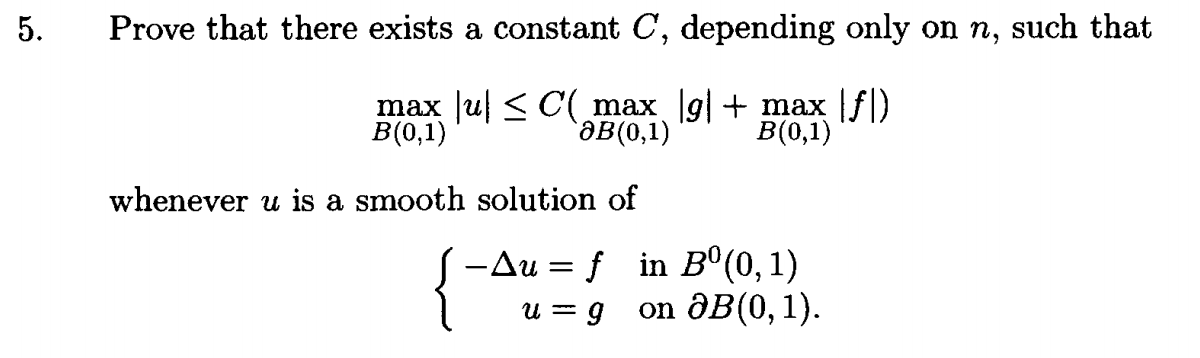
\includegraphics[width=0.8\textwidth]{evans-2-5.png}
\end{figure}
\end{question}

\begin{solution}
\end{solution}
\newpage

\begin{question}[2-6]
\hfill
\begin{figure}[h!]
  \centering
    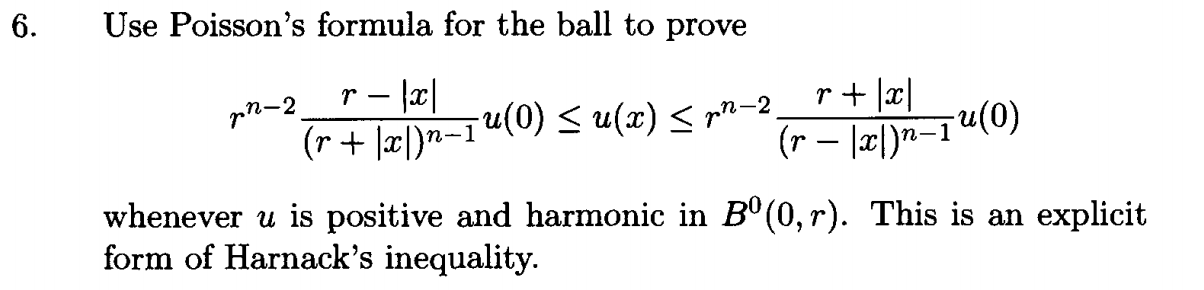
\includegraphics[width=0.8\textwidth]{evans-2-6.png}
\end{figure}
\end{question}

\begin{solution}
Fix $x \in B^0(0,r)$. If $y \in \partial B(0,r)$, then $|x-y| \leq x + r$, so
\eQb
u(x) &=& \dfrac{r^2 - |x|^2}{n \alpha(n) r} \int_{\partial B(0,r)} 
\dfrac{g(y)}{|x-y|^n} dS(y) 
\geq \dfrac{r^2 - |x|^2}{n \alpha(n) r} \int_{\partial B(0,r)} 
\dfrac{g(y)}{(|x|+r)^n} dS(y) \\
&=& r^{n-2} \dfrac{r - |x|}{(r+|x|)^{n-1}} \dfrac{1}{n\alpha(n) r^{n-1}} 
\int_{\partial B(0,r)} g(y) dS(y)  
= r^{n-2} \dfrac{r - |x|}{(r+|x|)^{n-1}}  
\Xint-_{\partial B(0,r)} g(y) dS(y) \\ 
&=& r^{n-2} \dfrac{r - |x|}{(r+|x|)^{n-1}}  
u(0)
\\ 
\eQe
\end{solution}

\newpage

\begin{question}[2-7]
\hfill
\begin{figure}[h!]
  \centering
    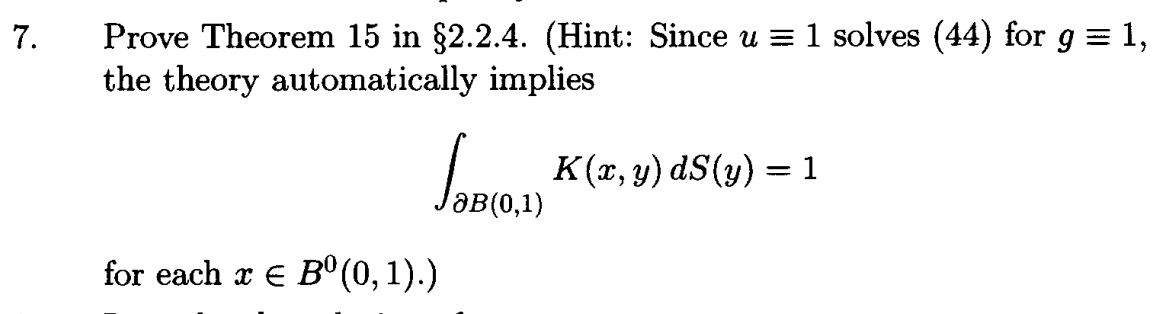
\includegraphics[width=0.8\textwidth]{evans-2-7.png}
\end{figure}
\end{question}

\begin{solution}
\end{solution}

\newpage

\begin{question}[2-8]
\hfill
\begin{figure}[h!]
  \centering
    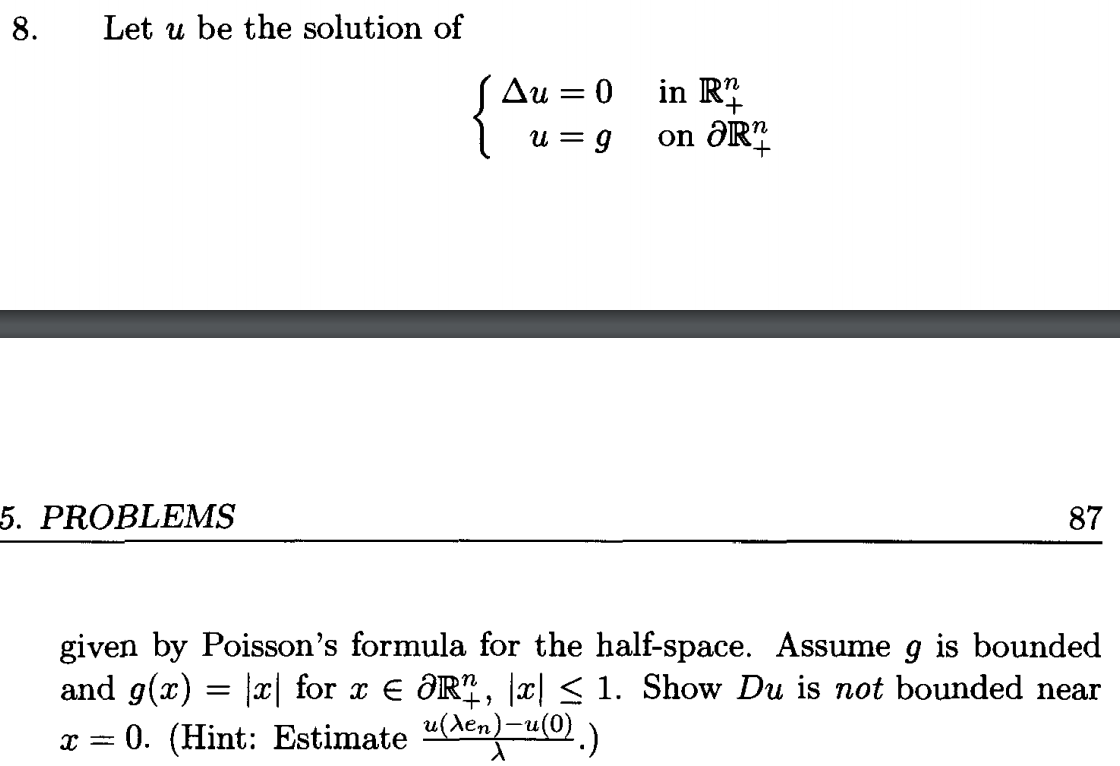
\includegraphics[width=0.8\textwidth]{evans-2-8.png}
\end{figure}
\end{question}

\begin{solution}
\end{solution}
\newpage

\begin{question}[2-9]
\hfill
\begin{figure}[h!]
  \centering
    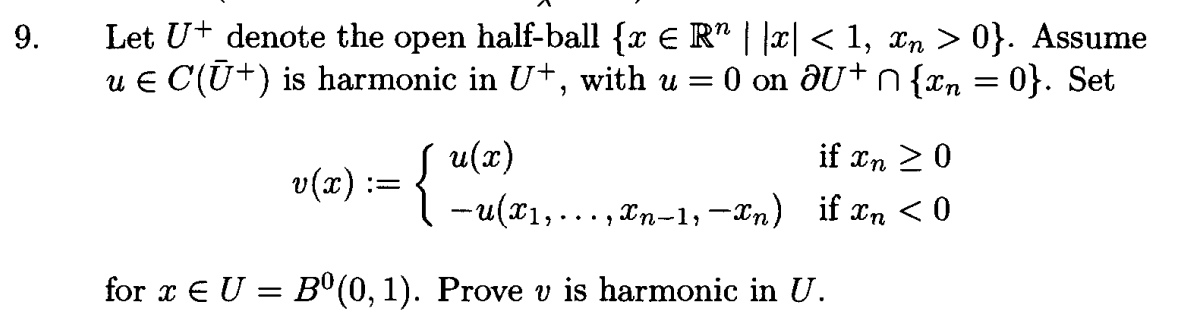
\includegraphics[width=0.8\textwidth]{evans-2-9.png}
\end{figure}
\end{question}

\begin{solution}
\end{solution}

\end{document}
